\section{Analysis of performance}

In order to reduce the interference due to other factors
during testing, benchmark testing has been proposed.
Benchmarking refers to the evaluation of
the performance of an object by running a computer program or
manipulating some specific behavior\cite{fleming1986not}.
It runs through a series of comparative experiments with controlled variables,
and it usually involves several iterative rounds in order to draw
reproducible and precise conclusions.
Next we will follow a benchmarking approach to quantitatively
analyze the performance of the programming language.

\subsection{Benchmarking Setup}

%\begin{table}[htb]
%    \centering
%    \caption{Benchmarking platform}
%    \label{tab:platform}
%    \begin{tabular}{cc}
%        \hline
%        CPU    & ECS 4 Cores 3.0GHz \\
%        Memory & 16GiB              \\
%        OS     & CentOS 8.2 64bit   \\
%        \hline
%    \end{tabular}
%\end{table}

This benchmarking uses Python scripts to perform coarse-grained batch testing
uniformly and uses the built-in process tools of Python to invoke Linux system
commands without relying on third-party libraries, which have high testing efficiency.
Each benchmarking runs six times with larger and smaller scale inputs,
and we process the results in some method respectively to avoid bias.
We choose the host with a 4-core 3.0GHz CPU, 16GB RAM, CentOS 8.2.
For the compiler environment of the programming language, see Table\ref{tab:version}.

\begin{table}[htbp]
    \caption{Language versions and dependencies}
    \label{tab:version}
    \begin{center}
        \begin{tabular}{ccc}
            \toprule
            Language   & Version         & Dependency \\
            \midrule
            Python     & CPython3.8      & -          \\
            Java       & OpenJDK17       & -          \\
            C++        & Clang14/GCC11.2 & -          \\
            JavaScript & Node16          & -          \\
            Go         & Go1.17          & -          \\
            Swift      & Swift5.5        & -          \\
            Dart       & Dart2.16        & -          \\
            Rust       & Rust1.54        & MinGW7.3   \\
            Kotlin     & Kotlin1.6       & OpenJDK8   \\
            \bottomrule
        \end{tabular}
    \end{center}
\end{table}

For the same language with different compilers or compilation methods (e.g.\ C++, Dart), compare their differences.
For the remaining languages, we classify them according to the type systems we discussed above.
Languages with the same type system and compilation method should have similar application scenarios,
so we should make a comparative analysis.

The benchmarking metrics for computer languages come from one of the
most popular cross-language benchmarking suites -
the Computer Language Benchmarking Game\cite{gouy2017computer}.
For each language, there are four metrics, and we will use them
in Table~\ref{tab:binary-trees}, Table~\ref{tab:n-body}, and Table~\ref{tab:mandelbrot} soon.
There are the details of these four metrics below.

\begin{enumerate}
    \item Compiler.
    Marked after the programming language.
    If not marked, we use the official compiler.
    \item Size.
    The size of the source code after gzip compression.
    The less code a programming language uses, the more expressive the language is for the same algorithm, in general.
    \item CPU. The time required to run the algorithm.
    Takes the minimum value of multiple runs.
    Includes startup time.
    \item Memory.
    The peak space consumption to run the algorithm.
    Takes the maximum of multiple runs.
\end{enumerate}

\subsection{Memory allocation test}
This algorithm is derived from Hans-J. Boehm's GC bench.
The memory allocation capacity and garbage collection capacity of a programming languages
are measured by repeatedly allocating and deallocating large amounts of space.
The steps are described in Algorithm 1.
We obtain the CPU and memory overhead results for the selected MPLs
by taking n=21 and n=14 respectively, as shown in Table~\ref{tab:binary-trees}.

\begin{figure}[htbp]
    \centerline{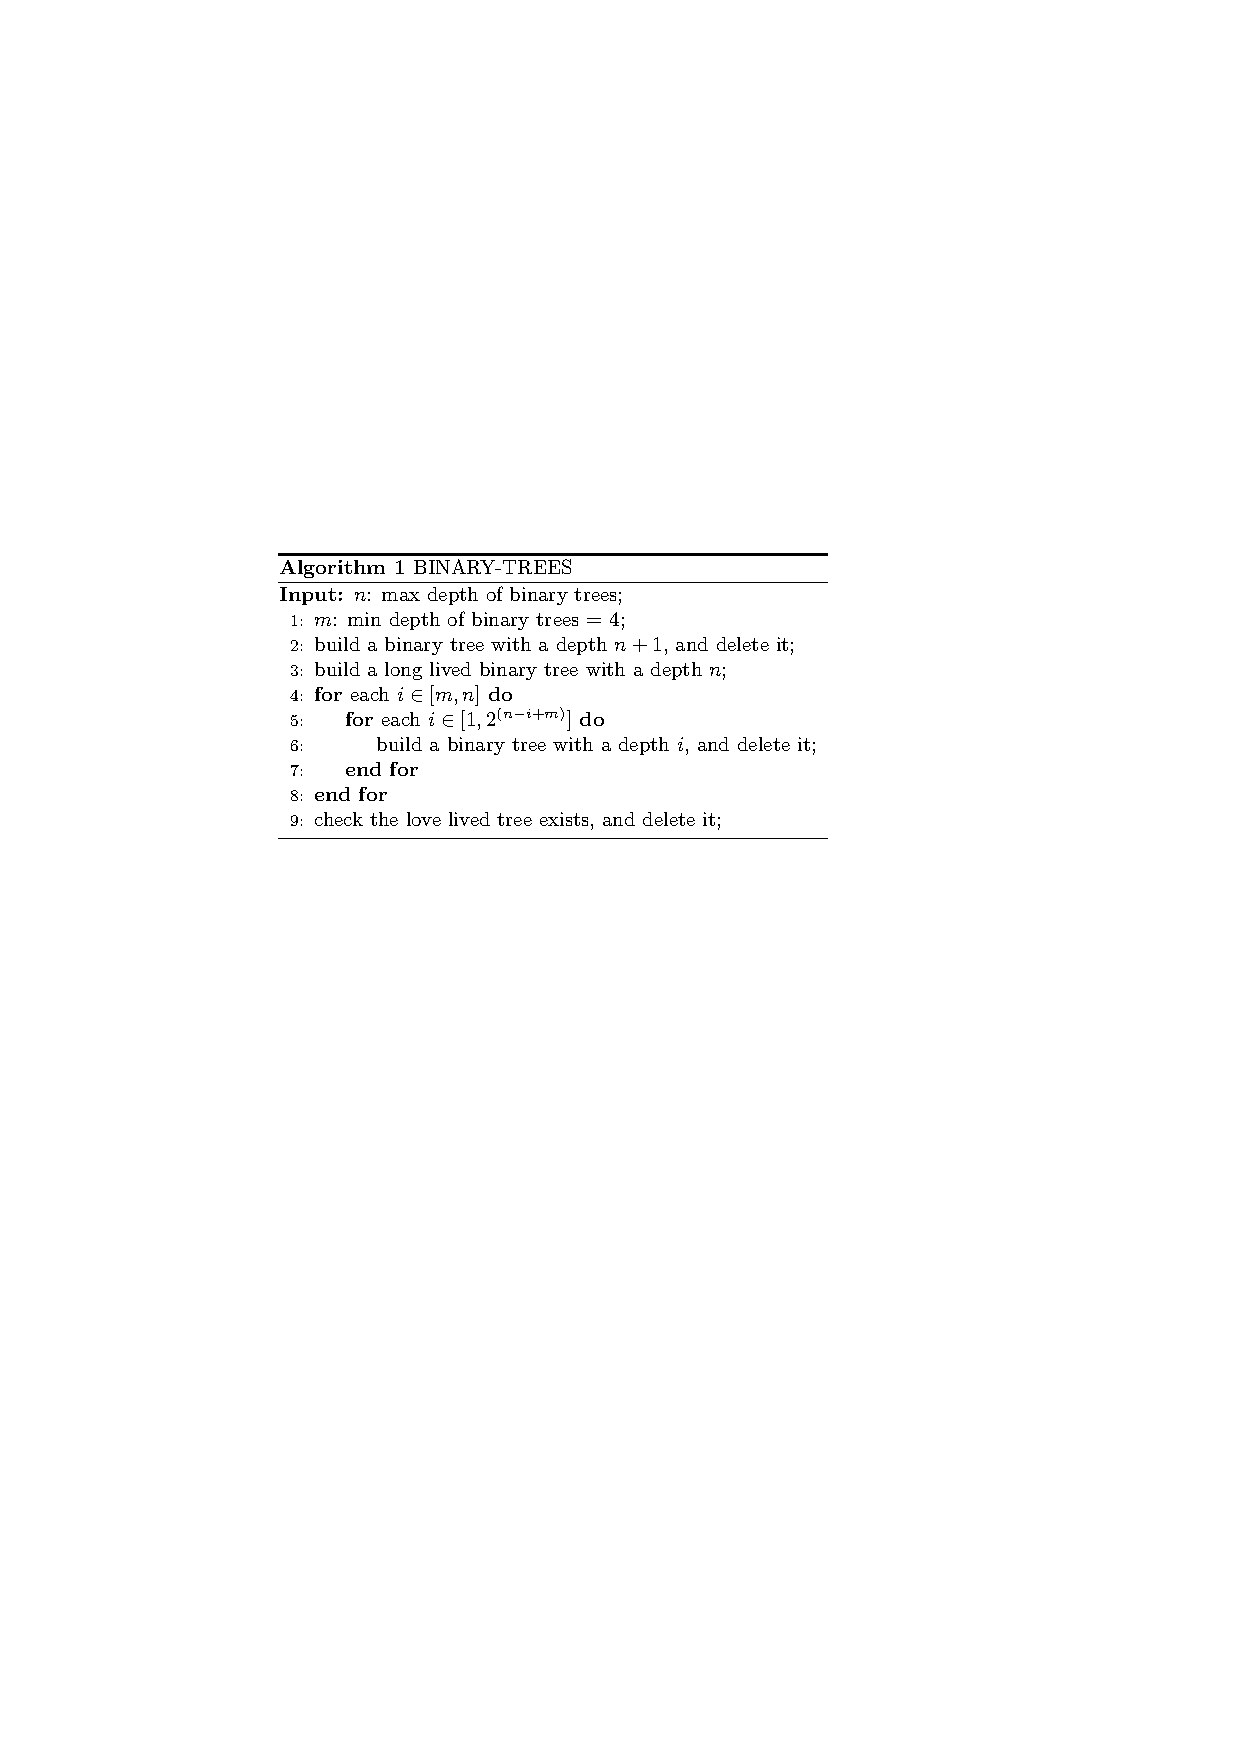
\includegraphics[scale=0.8]{figures/binary-trees}}
    \label{fig:binary-trees}
\end{figure}


\begin{table*}[htbp]
    \centering
    \caption{Memory allocation test}
    \label{tab:binary-trees}
    \begin{subtable}[h]{0.495\linewidth}
        \centering
        \begin{tabular}{lrrrr}
            \toprule
            lang      & n  & size(B) & cpu(s)  & mem(KB) \\
            \midrule
            cpp-clang & 21 & 654     & 16.438  & 263580  \\
            cpp-gcc   & 21 & 654     & 22.181  & 263620  \\
            dart-aot  & 21 & 1212    & 45.461  & 799012  \\
            dart-jit  & 21 & 1212    & 61.531  & 1626352 \\
            go        & 21 & 482     & 50.955  & 220548  \\
            java      & 21 & 552     & 5.607   & 2015512 \\
            js-node   & 21 & 711     & 36.391  & 1130788 \\
            kt-jvm    & 21 & 494     & 8.923   & 1783144 \\
            python3   & 21 & 589     & 169.912 & 442180  \\
            rust      & 21 & 751     & 7.796   & 132508  \\
            swift     & 21 & 714     & 63.608  & 733144  \\
            \bottomrule
        \end{tabular}
        \caption{Memory allocation test - large input}
        \label{tab:binary-trees-1}
    \end{subtable}
    \begin{subtable}[h]{0.495\linewidth}
        \centering
        \begin{tabular}{lrrrr}
            \toprule
            lang      & n  & size(B) & cpu(s) & mem(KB) \\
            \midrule
            cpp-clang & 14 & 654     & 0.087  & 1200    \\
            cpp-gcc   & 14 & 654     & 0.104  & 3928    \\
            dart-aot  & 14 & 1212    & 0.120  & 1680    \\
            dart-jit  & 14 & 1212    & 0.644  & 170008  \\
            go        & 14 & 482     & 0.214  & 7232    \\
            java      & 14 & 552     & 0.155  & 47968   \\
            js-node   & 14 & 711     & 0.717  & 90512   \\
            kt-jvm    & 14 & 494     & 0.249  & 36040   \\
            python3   & 14 & 589     & 0.911  & 14420   \\
            rust      & 14 & 751     & 0.042  & 1176    \\
            swift     & 14 & 714     & 0.299  & 17616   \\
            \bottomrule
        \end{tabular}
        \caption{Memory allocation test - small input}
        \label{tab:binary-trees-2}
    \end{subtable}
\end{table*}

As we can see from the Table\ref{tab:binary-trees},
Java has the best memory allocation and management
speed among these programming languages.
However, Java's memory consumption is relatively the largest among these languages.
This is due to the unique memory model of the JVM, which divides the heap area into
different generations and uses different garbage collection algorithms for each generation.
The advantage of this is obvious, it can greatly increase the efficiency of garbage
collection.
But at the same time, it takes up more memory than the storage of objects actually needs.
Since Kotlin and Java are both based on the JVM, they have similar performance figures.
Kotlin is based on Java8, while Java is based on Java17.
From Java9 onwards, the default JVM GC is G1.
It has a better response time than Parallel in Java8, but consumes more memory.
The performance impact of the GC can be seen from the Table\ref{tab:binary-trees}.
Kotlin's time overhead is slightly higher than Java's, and memory overhead is slightly lower.

In Table~\ref{tab:binary-trees},
for the two different compilers for C++, Clang and GCC, the memory overhead is almost the same.
This is largely because both of them manage memory manually.
However, Clang has a lower time overhead than GCC. These results are likely to be related to their
different compiler architecture and optimization.
In fact, the architecture of the two compilers is different:
Clang-LLVM uses a low-coupling front- and back-end architecture, while GCC uses a front- and back-end coupling
architecture.
We can see that compile-time optimization of the compiler takes a significant role for natively compiled languages.

Rust, Go and Swift, which are also strongly checked, natively compiled MPLs,
use three different memory management models.
The test results in Table~\ref{tab:binary-trees} for the three are highly dependent on their
respective memory models.
Go uses a garbage collector.
Although Go is a natively compiled language, there is an additional runtime to support garbage collection.
Compared to Java, Go uses a more conservative garbage collection strategy
resulting in decent space consumption and less optimistic runtimes for memory
allocation in Table~\ref{tab:binary-trees}.
Rust uses an ownership mechanism,
unlike C/C++, which is purely manually managed, and unlike Go's garbage collection.
In terms of the underlying implementation, Rust does not actually maintain a runtime
to manage memory but rather determines the timing of unallocating memory at compile
time through a complex ownership algorithm.
As a result, Rust's memory management is overhead-free.
In fact, Rust's compiler backend uses LLVM, the same
backend as the Clang-LLVM tested above.
And it is also clear from the data in Table~\ref{tab:n-body} that
Rust performs almost identically to Cpp-Clang.
Due to its ownership mechanism, Rust is the best at memory allocation in selected MPLs.
For Swift, the memory management mechanism is different from all of the above.
Swift allocates and deallocates memory by maintaining a runtime reference count.
In addition, Swift forces reference counts to be updated atomically for thread safety,
which results in higher CPU and memory overhead than Rust in Table~\ref{tab:binary-trees}.
This shows that Swift has a higher runtime overhead compared to Rust.

\subsection{Floating-point operation test}

This algorithm comes from the Symplectic Integration algorithm of K. P. Rauch and D. P. Hamilton.
They simulates the evolution of multiple planets and checks the correctness of the program
by examining the energy of each evolutionary state.
The performance bottleneck of this algorithm is mainly in floating-point operations.
The steps are described in Algorithm 2.
We obtain the CPU and memory overhead results
for the selected MPLs by taking n=5e7 and n=5e6, respectively,
as shown in Table~\ref{tab:n-body}.

\begin{figure}[htbp]
    \centerline{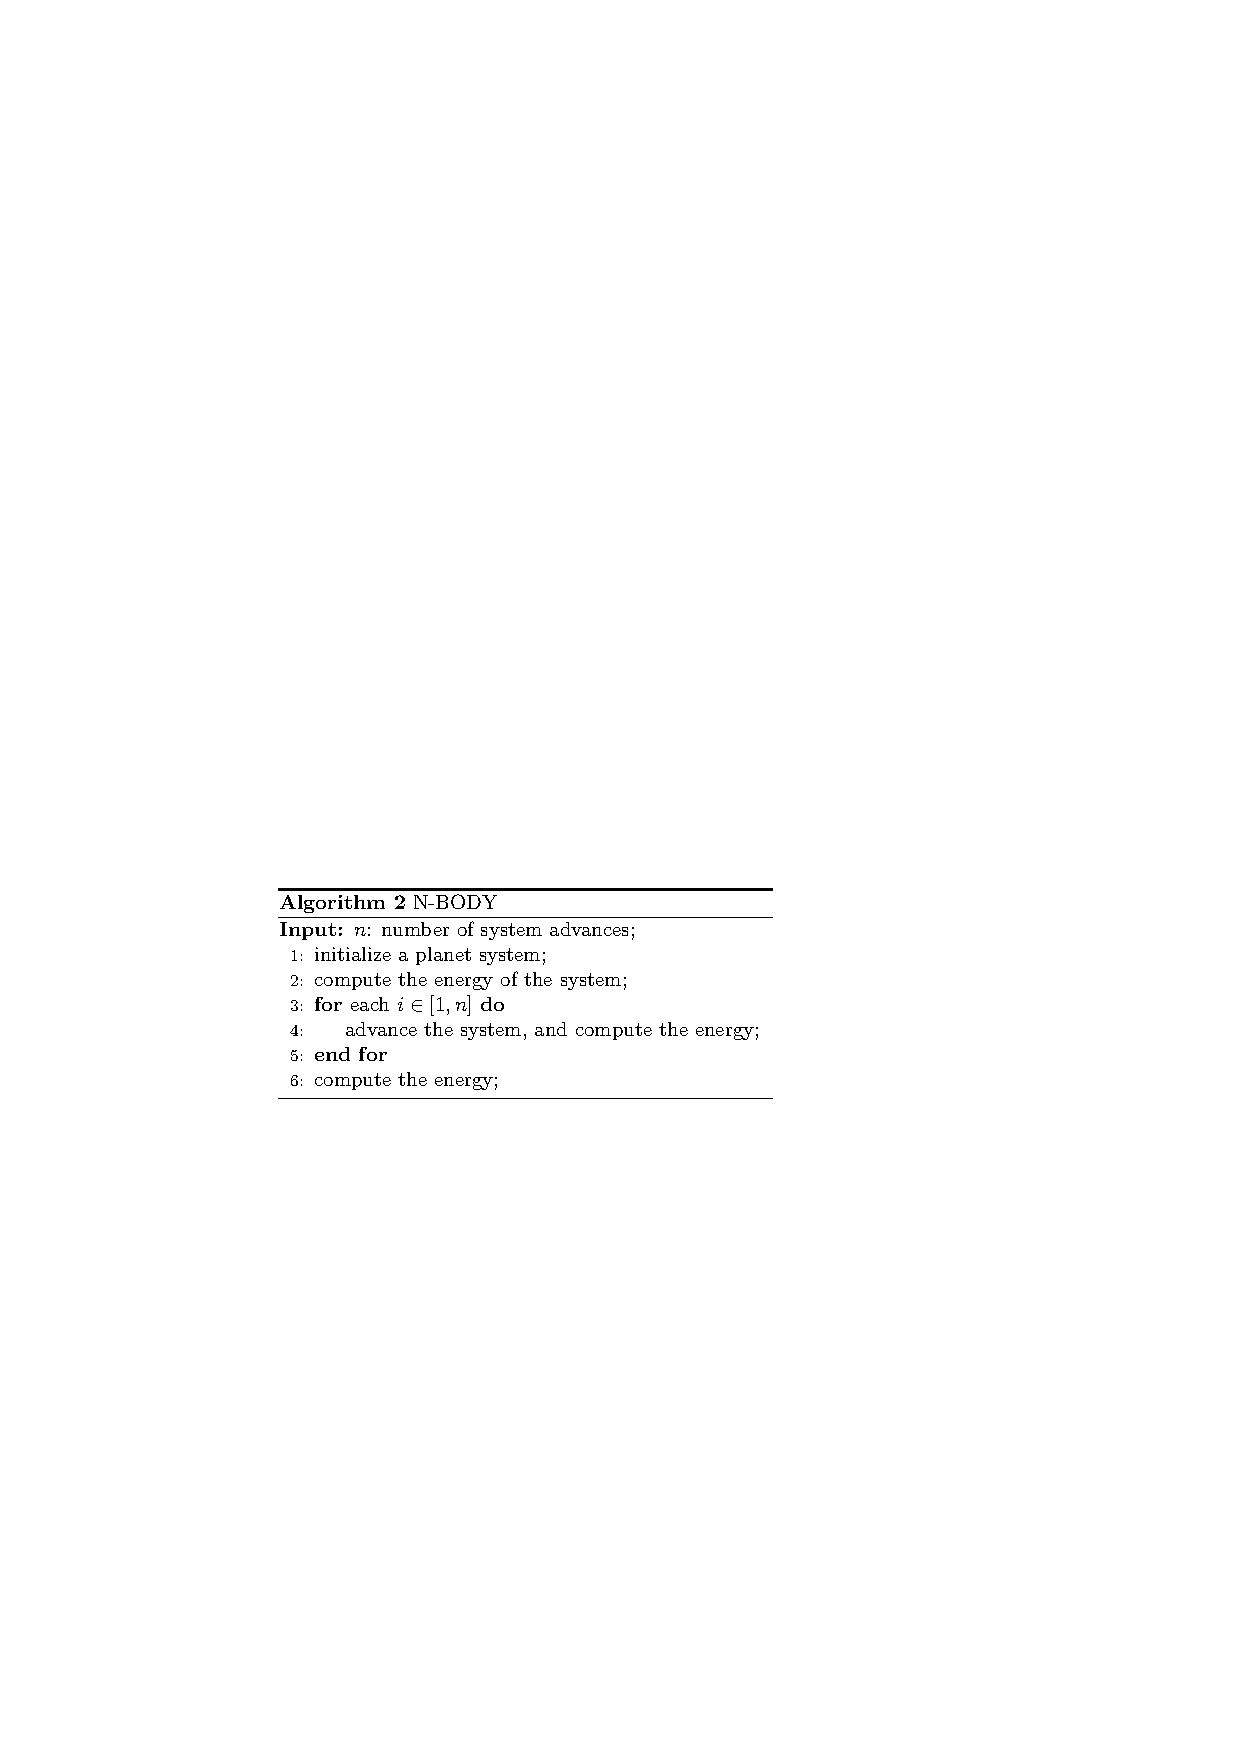
\includegraphics[scale=0.8]{figures/n-body}}
    \label{fig:n-body}
\end{figure}

\begin{table*}[htbp]
    \centering
    \caption{Memory allocation test}
    \label{tab:n-body}
    \begin{subtable}[h]{0.495\linewidth}
        \centering
        \begin{tabular}{lrrrr}
            \toprule
            lang      & n        & size(B) & cpu(s)  & mem(KB) \\
            \midrule
            cpp-clang & 50000000 & 1173    & 5.926   & 1236    \\
            cpp-gcc   & 50000000 & 1173    & 7.555   & 1228    \\
            dart-aot  & 50000000 & 1266    & 10.220  & 9308    \\
            dart-jit  & 50000000 & 1266    & 13.193  & 143436  \\
            go        & 50000000 & 1310    & 6.581   & 1128    \\
            java      & 50000000 & 1430    & 7.816   & 37260   \\
            js-node   & 50000000 & 1268    & 8.550   & 39956   \\
            kt-jvm    & 50000000 & 1124    & 6.914   & 37068   \\
            python3   & 50000000 & 1196    & 541.319 & 7780    \\
            rust      & 50000000 & 1480    & 5.818   & 1024    \\
            swift     & 50000000 & 1192    & 9.585   & 6308    \\
            \bottomrule
        \end{tabular}
        \caption{Floating-point operation test - large input}
        \label{tab:n-body-1}
    \end{subtable}
    \begin{subtable}[h]{0.495\linewidth}
        \centering
        \begin{tabular}{lrrrr}
            \toprule
            lang      & n       & size(B) & cpu(s) & mem(KB) \\
            \midrule
            cpp-clang & 5000000 & 1173    & 0.621  & 1204    \\
            cpp-gcc   & 5000000 & 1173    & 0.766  & 1204    \\
            dart-aot  & 5000000 & 1266    & 1.033  & 9216    \\
            dart-jit  & 5000000 & 1266    & 1.918  & 143256  \\
            go        & 5000000 & 1310    & 0.661  & 816     \\
            java      & 5000000 & 1430    & 0.880  & 37460   \\
            js-node   & 5000000 & 1268    & 0.941  & 39864   \\
            kt-jvm    & 5000000 & 1124    & 0.826  & 37064   \\
            python3   & 5000000 & 1196    & 52.530 & 7800    \\
            rust      & 5000000 & 1480    & 0.579  & 1020    \\
            swift     & 5000000 & 1192    & 0.976  & 6308    \\
            \bottomrule
        \end{tabular}
        \caption{Floating-point operation test - small input}
        \label{tab:n-body-2}
    \end{subtable}
\end{table*}

As shown in Table~\ref{tab:binary-trees},
Java's time overhead is not very high and does not fall too far behind natively compiled languages.
The performance bottleneck of JVM-based programs with short execution time is mainly the JVM startup
time and the JIT-optimized warm-up time, and for algorithms that have already done so,
Java's execution speed does not lag behind that of natively compiled languages.
Java runs in two steps.
In the first step, the source code is compiled into bytecode, and in the second step,
the JVM interprets and executes the bytecode.
In the process of interpreting and executing the bytecode, JVM will analyze the runtime
information of the bytecode, and if it finds that some bytecode is executed more frequently,
it will compile this part of the bytecode into native code.
Then if programs want to execute bytecode, JVM will first check if there is compiled native code and execute it.
The so-called performance optimization of Java is mainly in the bytecode stage,
while the source code to bytecode stage is only a simple optimization.

Table~\ref{tab:binary-trees} presents the significant performance gap between JavaScript and Python.
They are both so-call scripting language (a part of interpreted language),
and they interpret source code line by line and execute directly.
The performance of interpreted languages is closely related to the optimization of its interpreter.
JavaScript runs on Google's V8 engine, which executes JavaScript code much like the
JVM executes bytecode, using the JIT optimization technique.
So compared to Python, which does not use JIT optimization, it has a huge performance
improvement, even with Java and natively compiled languages with similar floating point performance.
In fact, the speed of scripting languages is not a performance bottleneck in most application scenarios.
However, in recent years, JavaScript has become the "assembly of the web",
and more and more languages are being compiled into JavaScript (e.g., Kotlin and Dart),
so more and more business logic needs to be executed in JavaScript.
This makes JavaScript burdened with tedious business-related logic, and optimization of JavaScript is the trend.
The application scenarios of Python are different from those of JavaScript.
Python is currently mainly used for scientific computing, data analysis and AI\@.
The performance of Python itself is relatively low, but most of the so-called Python libraries
only provide Python interfaces, and the underlying implementation is still other high-performance
languages (e.g., C).
This is also a way to improve performance.

\subsection{Comprehensive test}

The Mandelbrot Set is drawn on a resolution N×N image and the coordinates of the image on the complex axis are [-1.5-i,0.5+i].
For each pixel, a certain number of iterations are performed to determine the gray level of the current pixel.
Then program output in PBF format byte by byte.
Its correctness is checked by comparing its output with the standard output.
The performance bottleneck of this test is in floating point operations, memory allocation, and IO\@.
The steps are described in Algorithm 3.
We obtain the CPU and memory overhead results for the selected MPLs by taking n=16000 and n=4000, respectively,
as shown in Table~\ref{tab:mandelbrot}.

\begin{figure}[htbp]
    \centerline{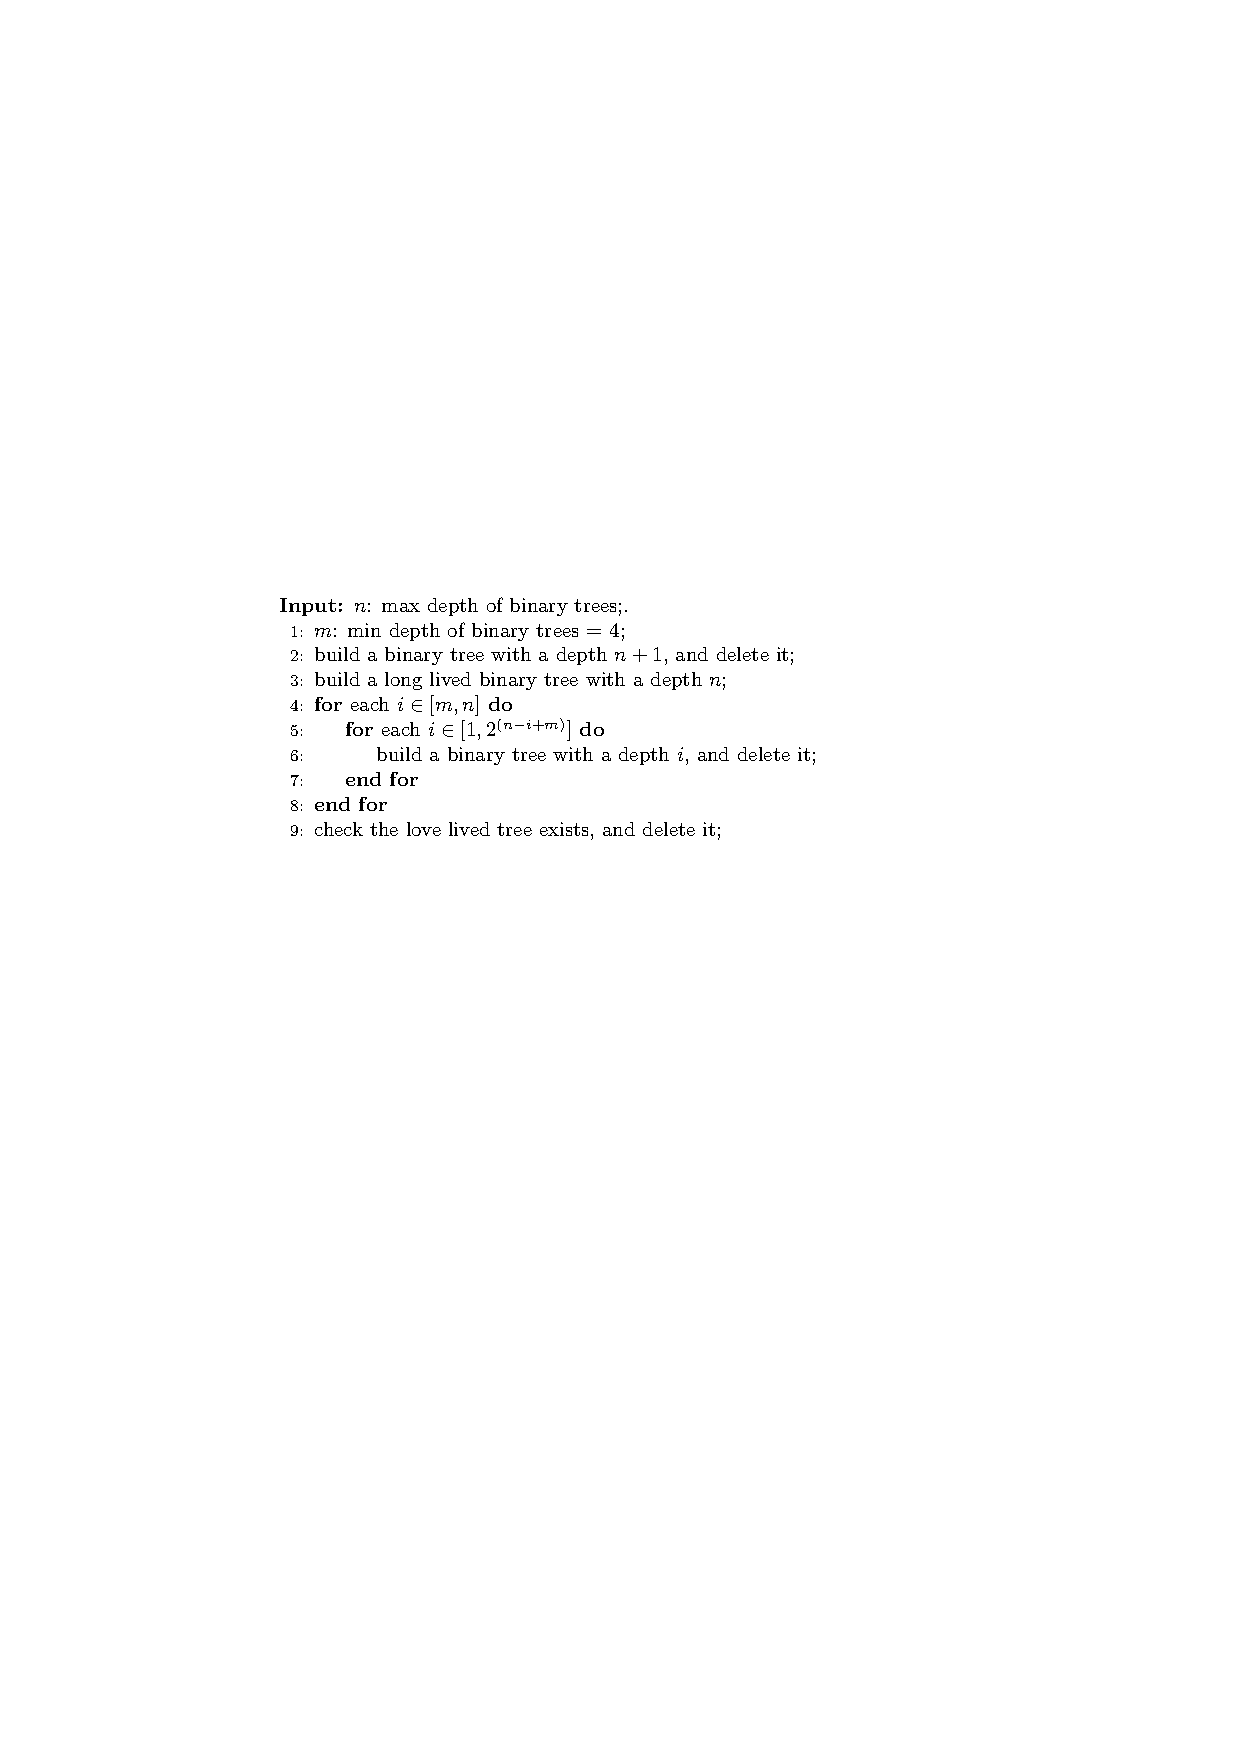
\includegraphics[scale=0.8]{figures/mandelbrot}}
    \label{fig:mandelbrot}
\end{figure}


\begin{table*}[htbp]
    \centering
    \caption{Memory allocation test}
    \label{tab:mandelbrot}
    \begin{subtable}[h]{0.495\linewidth}
        \centering
        \begin{tabular}{lrrrr}
            \toprule
            lang      & n     & size(B) & cpu(s)  & mem(KB) \\
            \midrule
            cpp-clang & 16000 & 822     & 13.900  & 30172   \\
            cpp-gcc   & 16000 & 822     & 13.931  & 28696   \\
            dart-aot  & 16000 & 454     & 154.089 & 17240   \\
            dart-jit  & 16000 & 454     & 151.501 & 148144  \\
            go        & 16000 & 823     & 19.598  & 32412   \\
            java      & 16000 & 665     & 27.834  & 34264   \\
            js-node   & 16000 & 373     & 130.638 & 42020   \\
            kt-jvm    & 16000 & 407     & 30.032  & 28432   \\
            python3   & 16000 & 688     & 702.599 & 47780   \\
            rust      & 16000 & 868     & 11.904  & 38528   \\
            swift     & 16000 & 394     & 26.277  & 6200    \\
            \bottomrule
        \end{tabular}
        \caption{Comprehensive test - large input}
        \label{tab:mandelbrot-1}
    \end{subtable}
    \begin{subtable}[h]{0.495\linewidth}
        \centering
        \begin{tabular}{lrrrr}
            \toprule
            lang      & n    & size(B) & cpu(s) & mem(KB) \\
            \midrule
            cpp-clang & 4000 & 822     & 0.880  & 1552    \\
            cpp-gcc   & 4000 & 822     & 0.881  & 1192    \\
            dart-aot  & 4000 & 454     & 10.276 & 17380   \\
            dart-jit  & 4000 & 454     & 10.096 & 148084  \\
            go        & 4000 & 823     & 1.260  & 2420    \\
            java      & 4000 & 665     & 1.827  & 34352   \\
            js-node   & 4000 & 373     & 8.763  & 42540   \\
            kt-jvm    & 4000 & 407     & 2.419  & 28448   \\
            python3   & 4000 & 688     & 46.273 & 12172   \\
            rust      & 4000 & 868     & 0.757  & 4388    \\
            swift     & 4000 & 394     & 1.661  & 6240    \\
            \bottomrule
        \end{tabular}
        \caption{Comprehensive test - small input}
        \label{tab:mandelbrot-2}
    \end{subtable}
\end{table*}

For the same Dart code, it has two different ways of compiling, JIT and AOT\@.
Both ways have similar time overhead and memory overhead in the Table~\ref{tab:mandelbrot}.
This is caused by the compilation mechanism of Dart official compilers.
In fact, the running mechanism of Dart is different from the traditional way that JIT in JavaScript or AOT in Cpp.
The traditional AOT is to compile the source code directly into the object code on the target machine,
which can be called and run independently by the operating system directly.
However, for Dart, whether its compilation method is AOT or JIT, only their compilation time is different,
and they will eventually run on the virtual machine.
In fact, when the compilation time overhead is negligible, the time overhead of AOT and JIT is approximately equal.
And this way of running has its unique features.
It will significantly increase the running overhead of AOT mode, but this makes AOT compilation has strong runtime support.
Because of this feature, the Dart VM can save the current runtime state, and when the next time VM is started,
it can directly load the last state without startup.
And the incremental compilation allows Dart to recompile only a small amount of code when the code changes.
Dart is mainly for the front-end cross-platform framework Flutter.
With such hot reload and incremental compilation, code changes of Dart can feed back to the UI in real-time,
which is hard to do with other languages.
So developers could have a better development experience with Dart.

In industrial applications, the performance bottleneck in most scenarios is compile-related,
including not only compile-time but also run-time.
The impact of compilation on programming language efficiency is also multifaceted.
First, the same programming language with different compilers will often have different object codes,
which results in different runtime efficiency.
This is often due to different compile-time optimizations;
for example, for C++, there is a significant performance advantage in object codes obtained by compiling
with Clang-LLVM as opposed to compiling with GCC\@.
Second, the same programming language can run not only in AOT, but also in JIT\@.
For example, for Kotlin, it can be compiled not only to bytecode to run on JVM, but also JavaScript code to run on the browser.
Or even Kotlin can be compiled to native code, which directly run on the OS\@.
In this way, the different compilation methods have a greater impact on efficiency of a language.

The impact of memory management on programming language performance is huge too.
First, there is the matter of memory allocation on the heap.
For languages with VM, memory allocation is an advantage compared to non-VM languages.
Developers can focus on business logic without worrying about memory management.
VM languages provide memory pools that host the memory allocation, whereas non-VM languages do not.
Of course, under some scenarios, there is a frequently memory allocation on the heap,
non-VM languages tend to use custom or third-party memory pooling frameworks,
and the performance gap between VM and non-VM languages in the industry is not as pronounced.
But managed memory is not always an advantage.
When a memory thrash occurs, the VM will frequently GC, which greatly affects performance.
And, managed memory tend to have a larger memory overhead than they actually need (e.g., Java).
Second, there is the Principle of Locality about memory.
CPU will put all the adjacent data into cache, and if the memory is accessed sequentially,
it greatly improves the hit rate of cache, thus improving the performance.
